\documentclass{article} % For LaTeX2e
\usepackage{nips15submit_e,times}
\usepackage{hyperref}
\usepackage{url}
%\documentstyle[nips14submit_09,times,art10]{article} % For LaTeX 2.09

\usepackage{amsmath}
\usepackage{graphicx}
\usepackage{listings}             % Include the listings-package
\lstset{language=Python}          % Set your language (you can change the language for each code-block optionally)

\title{CSE253 Homework 1  \\ Enroll date : 9pm 15 Jan. }


\author{
David S.~Hippocampus\\
Department of Computer Science\\
Cranberry-Lemon University\\
Pittsburgh, PA 15213 \\
\texttt{hippo@cs.cranberry-lemon.edu}
}

% The \author macro works with any number of authors. There are two commands
% used to separate the names and addresses of multiple authors: \And and \AND.
%
% Using \And between authors leaves it to \LaTeX{} to determine where to break
% the lines. Using \AND forces a linebreak at that point. So, if \LaTeX{}
% puts 3 of 4 authors names on the first line, and the last on the second
% line, try using \AND instead of \And before the third author name.

\newcommand{\fix}{\marginpar{FIX}}
\newcommand{\new}{\marginpar{NEW}}

%\nipsfinalcopy % Uncomment for camera-ready version

\begin{document}


\maketitle


\section{Problems from Bishop}


\subsection{}

\begin{equation}
    \begin{array}{rcl}
        \prod\limits_{i = 1}^{d}\int_{-\infty}^{\infty}e^{-x_i^2} d x_i& = & S_d\int_{0}^{\infty}e^{-r^2}r^{d-1}dr\\
                S_d  & = & \frac{\prod\limits_{i = 1}^{d}\int_{-\infty}^{\infty}e^{-x_i^2} d x_i}{\int_{0}^{\infty}e^{-r^2}r^{d-1}dr}
    \end{array}
\end{equation}

According to (1.41),  we have
\begin{equation}
    \begin{array}{rcl}
       \int_{-\infty}^{\infty} exp\{-\frac{2}{\lambda}x^2\} dx  & =  & (\frac{2\pi}{\lambda})^{1/2}
    \end{array}
\end{equation}

In (2), we set $\lambda = 2$, we can get

\begin{equation}
    \begin{array}{rcl}
       \int_{-\infty}^{\infty} e^{-x^2} dx  & =  & \pi^{1/2} \\
        \prod\limits_{i = 1}^{d}\int_{-\infty}^{\infty}e^{-x_i^2} d x_i& = & \pi^{d/2} \\
    \end{array}
\end{equation}

According to (1.44),  we have
\begin{equation}
    \begin{array}{rcl}
      	\Gamma(x) \equiv \int_{0}^{\infty}u^{x-1}e^{-u} du
    \end{array}
\end{equation}

In (4), we set $u = r^2$, we can get

\begin{equation}
    \begin{array}{rcl}
      	\Gamma(x) \equiv \int_{0}^{\infty}r^{2(x-1)}e^{-r^2} dr^2 \equiv 2\int_{0}^{\infty}r^{2x-1}e^{-r^2} dr
    \end{array}
\end{equation}

In (5), set $d= 2x$

\begin{equation}
    \begin{array}{rcl}
      	\Gamma(\frac{d}{2})  \equiv 2\int_{0}^{\infty}r^{d-1}e^{-r^2} dr
    \end{array}
\end{equation}

Put (3) and (6) into (1),we can get

\begin{equation}
    \begin{array}{rcl}
     	S_d  & = & \frac{\prod\limits_{i = 1}^{d}\int_{-\infty}^{\infty}e^{-x_i^2} d x_i}{\int_{0}^{\infty}e^{-r^2}r^{d-1}dr} \\
	& = & \frac{2\pi^{d/2}}{\Gamma(\frac{d}{2})}
    \end{array}
\end{equation}

When $d = 2$,
\begin{equation}
    \begin{array}{rcl}
     	S_2  & = & \frac{2\pi^{d/2}}{\Gamma(\frac{d}{2})} \\
	& = & \frac{2\pi}{\Gamma(1)} \\
	& = & 2\pi
    \end{array}
\end{equation}

The area of circle is $\pi r ^ 2$

When $d = 3$,
\begin{equation}
    \begin{array}{rcl}
     	S_3  & = & \frac{2\pi^{d/2}}{\Gamma(\frac{d}{2})} \\
	& = & \frac{2\pi^{3/2}}{\Gamma(\frac{3}{2})} \\
	& = & 4\pi
    \end{array}
\end{equation}

The area of sphere is $\frac{4}{3} \pi r ^ 3$

%% \subsection{Double-blind reviewing}

%% This year we are doing double-blind reviewing: the reviewers will not know 
%% who the authors of the paper are. For submission, the NIPS style file will 
%% automatically anonymize the author list at the beginning of the paper.

%% Please write your paper in such a way to preserve anonymity. Refer to
%% previous work by the author(s) in the third person, rather than first
%% person. Do not provide Web links to supporting material at an identifiable
%% web site.

%%\subsection{Electronic submission}
%%
%% \textbf{THE SUBMISSION DEADLINE IS June 5, 2015. SUBMISSIONS MUST BE LOGGED BY
%% 23:00, June 5, 2015, UNIVERSAL TIME}

%% You must enter your submission in the electronic submission form available at
%% the NIPS website listed above. You will be asked to enter paper title, name of
%% all authors, keyword(s), and data about the contact
%% author (name, full address, telephone, fax, and email). You will need to
%% upload an electronic (postscript or pdf) version of your paper.

%% You can upload more than one version of your paper, until the
%% submission deadline. We strongly recommended uploading your paper in
%% advance of the deadline, so you can avoid last-minute server congestion.
%%
%% Note that your submission is only valid if you get an e-mail
%% confirmation from the server. If you do not get such an e-mail, please
%% try uploading again. 


\subsection{}

For a hypersphere with radius a and dimension d, the surface $S = S_d a ^{d-1}$. Assuming a small cube in unit sphere with length of side L. Then the area is $L^{d-1}$. If the radius is a, then the length of new cube is aL, the new corresponding area is $aL^{d-1}$ .

So 
\begin{equation}
    \begin{array}{rcl}
     	V_d  & = &\int_{0}^{a}  S_d r^{d-1} dr \\
	& = & \frac{S_d}{d} \int_{0}^{a} r^d dr \\
	& = & \frac{s_d a^d}{d}
    \end{array}
\end{equation}

\begin{equation}
    \begin{array}{rcl}
     	\frac{volume  \hspace{1mm} of  \hspace{1mm} Sphere}{volume  \hspace{1mm} of  \hspace{1mm} Cube} & = & \frac{2 \pi^{\frac{d}{2}}a^d}{\Gamma(d/2)d(2a)^d}   \\
	& = & \frac {\pi^{\frac{d}{2}}}{d2^{d-1}\Gamma(d/2)}
    \end{array}
\end{equation}

When $d \to \infty $

\begin{equation}
    \begin{array}{rcl}
     	\frac{volume  \hspace{1mm}of  \hspace{1mm}Sphere}{volume  \hspace{1mm}of  \hspace{1mm}Cube} & = & \frac {\pi^{\frac{d}{2}}}{d2^{d-1}\Gamma(d/2)} \\
	& = & {\frac{\pi e }{d/2 - 1}}^{d/2-1/2} \frac{e^{-1/2}}{d2^{d-1/2}}(substitute \hspace{1mm}\Gamma(d/2)) \\
	& = & 0 \cdot 0 (d \to \infty) \\
	& = & 0
    \end{array}
\end{equation}

Next, calculating  ratio of the distance from the centre of the
hypercube to one of the corners, divided by the perpendicular distance to
' one of the edges,

\begin{equation}
    \begin{array}{rcl}
     	\frac{Dis(corner)}{Dis(edge)} & = &\frac{\sqrt{\sum\limits_{i = 1}^{d}a^2}}{a} \\
	& = & \sqrt{d}
    \end{array}
\end{equation}

It is straight-forward to see when $d \to \infty$, this value goes to $\infty$

\subsection{}

\begin{equation}
    \begin{array}{rcl}
     	f & = & 1 - \frac{V_{a-\epsilon}}{V_a}  \\
	& = &  1 - \frac{{(a-\epsilon)}^{d}}{a^d}\\
	& = & 1 - (1-\frac{\epsilon}{a})^d
    \end{array}
\end{equation}

When $d \to \infty$

\begin{equation}
    \begin{array}{rcl}
     	\lim\limits_{d \to \infty}^{} f & = & \lim\limits_{d \to \infty}^{}  1 - (1-\frac{\epsilon}{a})^d \\
	& = & 1 - 0 \\
	& = & 1
    \end{array}
\end{equation}

When $\epsilon / a = 0.01$,

$f_{d=2} = 1 - 0.99^2 = 0.0199$ \\
$f_{d=10} = 1 - 0.99^{10} = 0.0956$ \\
$f_{d=1000} = 1 - 0.99^{1000} = 0.99996$ \\

When lies inside the radius a/2,

$f_{d=2} = 0.5^2 = 0.25$ \\
$f_{d=10} = 1 - 0.5^{10} = 0.000977$ \\
$f_{d=1000} = 1 - 0.5^{1000} \approx 0.00000$ \\


\subsection{}
In Problem 1.2, we have show that for a hypersphere with radius a and dimension d, the surface $S = S_d a ^{d-1}$. 

So, 

\begin{equation}
    \begin{array}{rcl}
      	\int_{shell}^{} p(x) dx & = & p(r) S_d r^{d-1} \epsilon \\
	& = & \rho (r) \epsilon
    \end{array}
\end{equation}

Next, we calculate the  single maximum point,

\begin{equation}
    \begin{array}{rcl}
      	\rho (r) & = & \frac{S_d r^{d-1}}{(2\pi \sigma ^ 2) ^ {1/2}} exp ( - \frac{r^2}{2 \sigma ^2} ) \\
	& \propto & r^{d-1} exp ( - \frac{r^2}{2 \sigma ^2} )  =  f(r)\\
    \end{array}
\end{equation}

We want to find the value of r to make f(r) reach maximum value, so

\begin{equation}
    \begin{array}{rcl}
      	\frac{df(r)}{dr} & = & [ (d-1)r^{d-2} - r^{d-1} \frac{r}{\sigma ^2} ] exp ( - \frac{r^2}{2 \sigma ^2} ) = 0 \\
	\Rightarrow  \hat{r}& = & \sigma \sqrt{d-1} \\
	\Rightarrow \hat{r} & \approx & \sigma \sqrt{d} (d \gg 1)
    \end{array}
\end{equation}

From equation (17), we have

\begin{equation}
    \begin{array}{rcl}
      	\rho (r) & \propto & r^{d-1} exp ( - \frac{r^2}{2 \sigma ^2} )  \\
	& = & exp((d-1)\ln{r} - \frac{r^2}{2 \sigma ^2}) \\
    \end{array}
\end{equation}

So, 

\begin{equation}
    \begin{array}{rcl}
      	\frac {\rho (\hat{r}+\epsilon)}{\rho ({\hat{r})}} & = & exp^{(d-1)\ln{(1 + \frac{\epsilon}{\hat{r}}}) - \frac{2\epsilon \hat{r} + \epsilon^2}{2\sigma^2} } \\
	& = & exp^{(d-1)(\frac{\epsilon}{\hat{r}} - \frac{\epsilon^2}{2\hat{r}^2} ) -  \frac{2\epsilon \hat{r} + \epsilon^2}{2\sigma^2} }  \\
	& = & exp^{- \frac{\epsilon^2}{\sigma^2} } (substitute \hspace{1mm} (d-1) \hspace{1mm} with (\frac{\hat{r}}{\sigma})^2)
    \end{array}
\end{equation}


\section{Perceptron}
\label{gen_inst}

\subsection{}

\begin{equation}
    \begin{array}{rcl}
      	y(x) & =  & 0 \\
	\Rightarrow &  \omega ^ T x - \theta  = 0 \\
	\Rightarrow & \omega_1 x_1 + \omega_2 x_2 - \theta = 0
    \end{array}
\end{equation}

The decision boundary line is $\omega ^ T x  =  \theta$

\begin{equation}
    \begin{array}{rcl}
      	l & = & \frac{ax_0 + by_0 + c}{\sqrt{a^2+b^2}} \\
	& = & \frac{c}{\sqrt{a^2+b^2}} \\
	& = & \frac {-\theta}{\lVert \omega \rVert} \\
	& = & \frac {-\omega_0}{\lVert \omega \rVert}
    \end{array}
\end{equation}

\subsection{}
(a) \\
Learning rule: If output is 1 and should be 0, then lower weights to active inputs and raise the threshold; 
If output is 0 and should be 1, then raise weights to active inputs and lower the threshold.

(b) \\

\begin{center}

\begin{tabular}{ | c | c | c | c | c | c | c |}
  \hline			
  $x_1$ & $x_2$ & Output & Teacher & $w_1$ & $w_2$ & Threshold ($\theta$) \\ \hline
  1 & 1 & 1 & 0 & -1 & -1 & 1 \\ \hline
  0 & 1 & 0 & 1 & -1 & 0 & 0 \\ \hline
  1 & 0 & 0 & 1 & 0 & 0 & -1 \\ \hline
  1 & 1 & 1 & 0 & -1 & -1 & 0 \\ \hline
  0 & 1 & 0 & 1 & -1 & 0 & -1 \\ \hline
  1 & 1 & 1 & 0 & -2 & -1 & 0 \\ \hline
  1 & 0 & 0 & 1 & -1 & -1 & -1 \\ \hline
\end{tabular}

\end{center}

$w_1 = -1, w_2 = -1, \theta = -1$

(c) \\
It is not unique. \\

For example, $w_1 = -2, w_2 = -1, \theta = -2$


\subsection{}
(i.) \\

The implementation is in the appendix.

The advantage of the z score transformation is that it takes into account both the mean value and the variability in a set of raw data.

(ii.) \\

Blue colour stand for setosa, red colour stands for versicolor.

Classes linearly separable in each of the feature spaces.  Because it is easy to find a boundary line in each figure below.

\begin{figure}[htbp] %  figure placement: here, top, bottom, or page
   \centering
   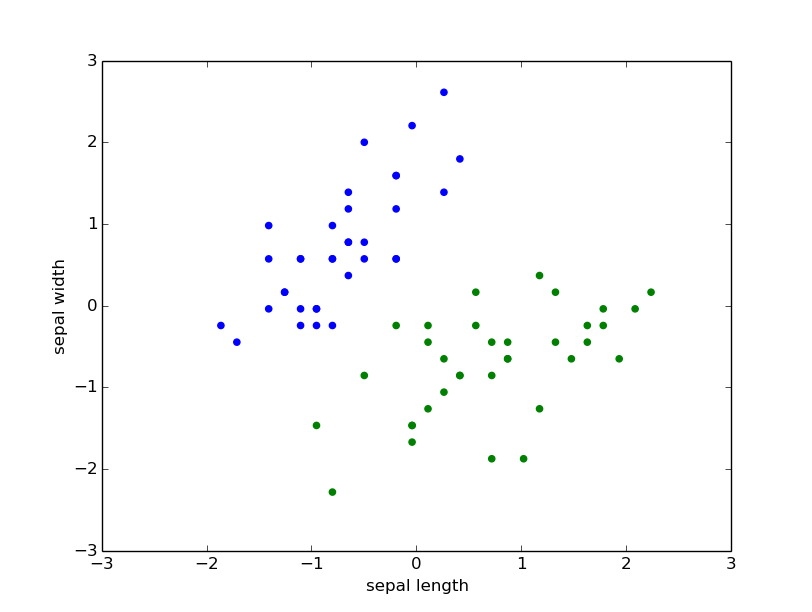
\includegraphics[width=3in]{img/figure1.png} 
\end{figure}

\begin{figure}[htbp] %  figure placement: here, top, bottom, or page
   \centering
   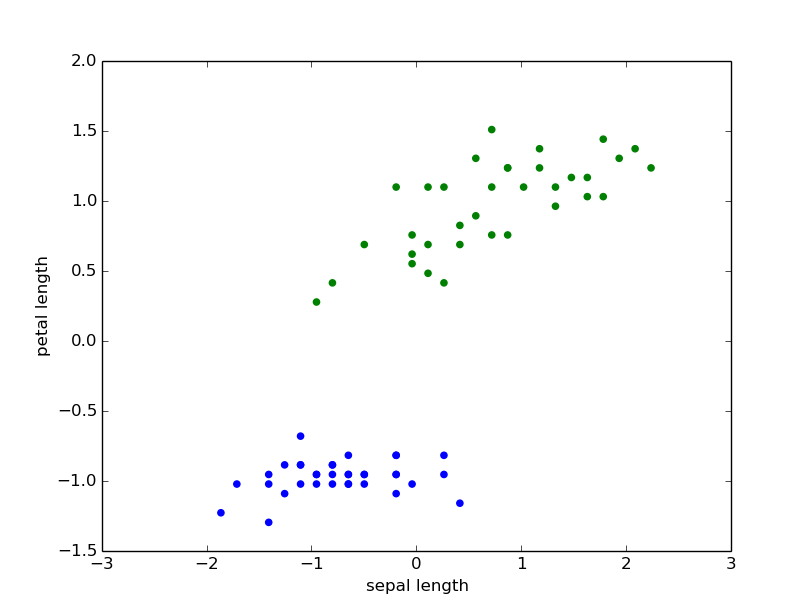
\includegraphics[width=3in]{img/figure2.png} 
\end{figure}

\begin{figure}[htbp] %  figure placement: here, top, bottom, or page
   \centering
   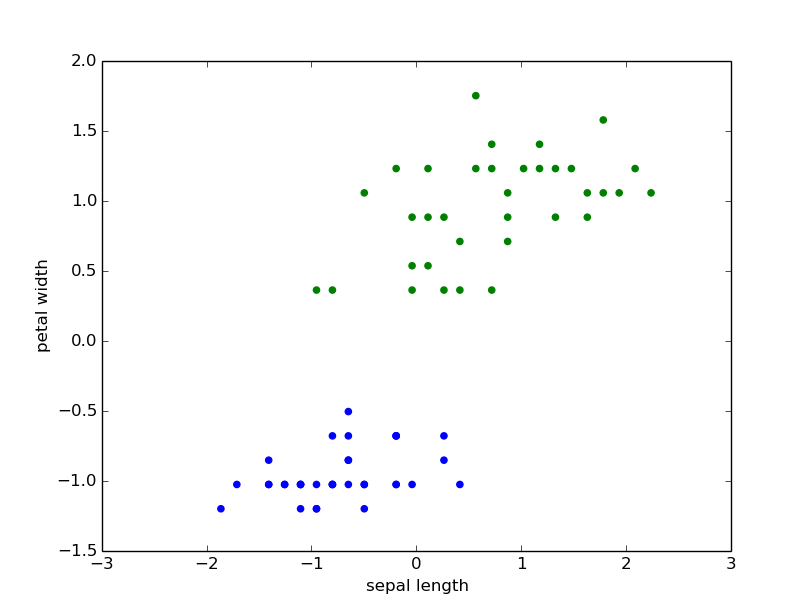
\includegraphics[width=3in]{img/figure3.png} 
\end{figure}

\begin{figure}[htbp] %  figure placement: here, top, bottom, or page
   \centering
   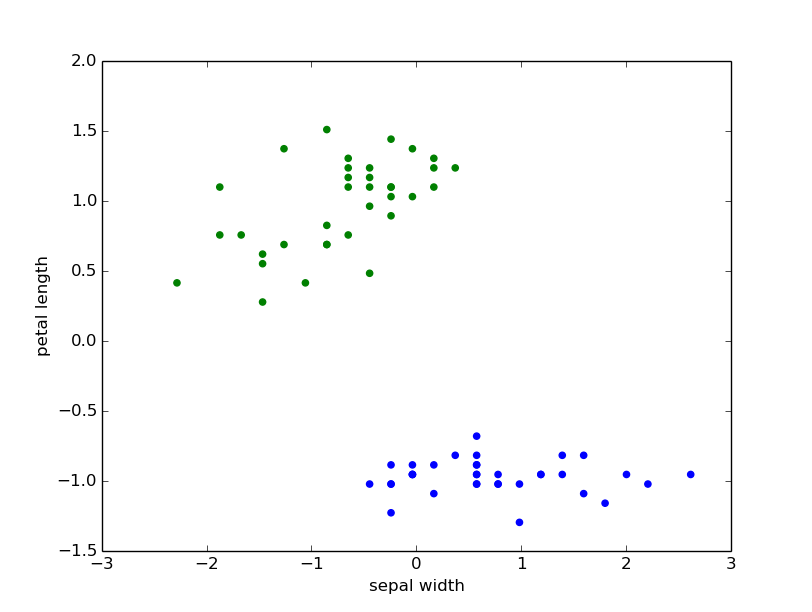
\includegraphics[width=3in]{img/figure4.png} 
\end{figure}

\begin{figure}[htbp] %  figure placement: here, top, bottom, or page
   \centering
   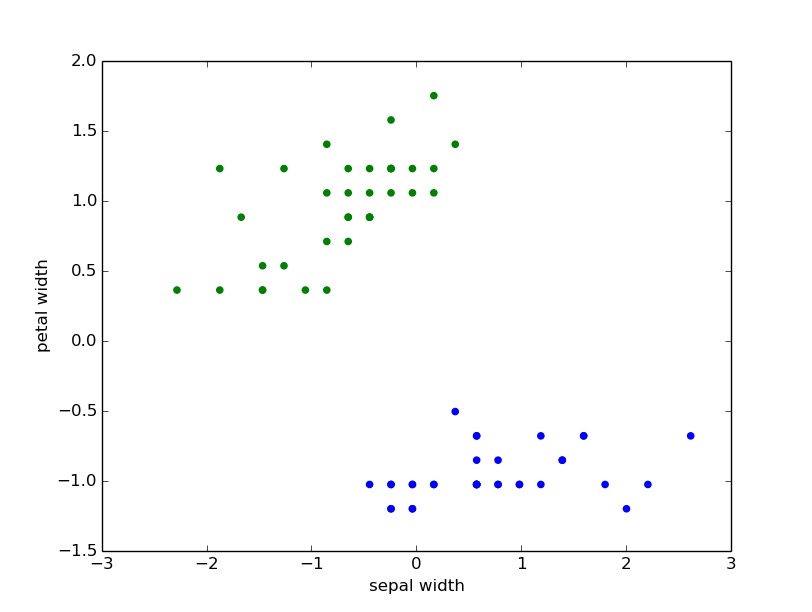
\includegraphics[width=3in]{img/figure5.png} 
\end{figure}

\begin{figure}[htbp] %  figure placement: here, top, bottom, or page
   \centering
   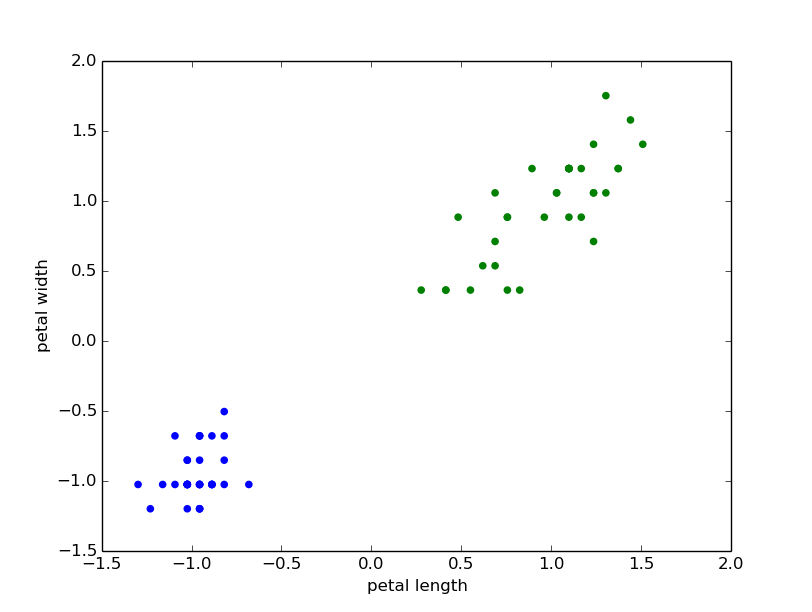
\includegraphics[width=3in]{img/figure6.png} 
\end{figure}

(iii.) \\
My source code is in the appendix.

(iv. v.) \\

\begin{center}

\begin{tabular}{ | c | c |}
  \hline			
  learning\_rate & error rate\\ \hline
  .25 & 0.0\% \\ \hline
  .5 & 0.0\% \\ \hline
  1.0 & 0.0\% \\ \hline
  2.0 & 0.0\% \\ \hline
\end{tabular}

\end{center}

For this test set, our model and prediction is very prefect. I run many times and each iteration always choose a random point and try different learning rate, all get 0.0\% error rate. So I think the data must be linearly separable. That is to say, the test data is very good.


\section{Logistic and Softmax Regression}

\subsection{}
\begin{equation}
    \begin{array}{rcl}
      	 - \frac{\partial{E^n(\omega)}}{\partial{\omega_j}} & = & \frac{t^n}{g_w(x^n)} \frac{\partial{g_w(x^n)}}{\partial \omega_j} - \frac{(1 - t^n)}{1 - g_w(x^n)} \frac{\partial{g_w(x^n)}}{\partial \omega_j} \\
	& = & t^n g_w(-x^n) x_j^n - (1 - t^n) g_w(x^n) x_j^n \\
	& = & x_j (-t^n(1 - y^n) + (1 - t^n)y^n)\\
	& = & (t^n - y^n)x_j
    \end{array}
\end{equation}

\subsection{}

First, 
$ \ln(\frac{a}{b}) = \ln{a} - \ln{b} \Rightarrow \ln{y_k^n} = a_k^n - \ln{\sum_{k'} exp(a_{k'}^n)}$

Then,

\begin{equation}
    \begin{array}{rcl}
      	 - \frac{\partial{E^n (\omega)} } { \partial{\omega_{jk}} } & = 
	 & \sum\limits_{m = 1}^{c} t_c^n \frac{\partial{\ln{y_m^n}} } {\partial{\omega_{jk}}} \\
	 & = &  \sum\limits_{m = 1}^{c} t_c^n \frac{\partial{  a_m^n - \ln{\sum_{k'} exp(a_{k'}^n)} } } {\partial{\omega_{jk}}} \\
	 & = & t_k^n(x_j^n - \frac{ exp(a_k^n) x_j^n}{ \sum_{k'} exp(a_{k'}^n) }  ) + \sum\limits_{m \not\equiv k} t_m^n(- \frac{ exp(a_k^n) x_j^n}{ \sum_{k'} exp(a_{k'}^n) } ) \\
	 & = & t_k^n x_j^n - \frac{ exp(a_k^n) x_j^n}{ \sum_{k'} exp(a_{k'}^n) }  \sum\limits_{m=1}^{c} t_m^n \\
	 & = & t_k^n x_j^n - \frac{ exp(a_k^n) x_j^n}{ \sum_{k'} exp(a_{k'}^n) }  \\
	 & = & (t_k^n - y _k^n) x_j^n
    \end{array}
\end{equation}

\subsection{}
The implementation is in appendix reference http://g.sweyla.com/blog/2012/mnist-numpy/.


\subsection{}
(a) \\

\begin{center}

\begin{tabular}{ | c | c |}
  \hline			
  Number & Accuracy \\ \hline
  0 & 98.3\% \\ \hline
  1 & 98.95\% \\ \hline
  2 & 97.3\% \\ \hline
  3 & 97.05\% \\ \hline
  4 & 97.4\% \\ \hline
  5 & 92.8\% \\ \hline
  6 & 97.8\% \\ \hline
  7 & 96.4\% \\ \hline
  8 & 91.9\% \\ \hline
  9 & 94.2\% \\ \hline

\end{tabular}

\end{center}

(b) \\
The overall accuracy is 82.25 \%


\section{Softmax Regression via Gradient Descent}

(a) \\
\begin{figure}[htbp] %  figure placement: here, top, bottom, or page
   \centering
   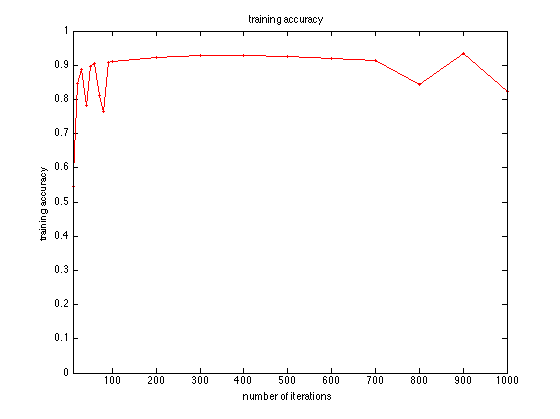
\includegraphics[width=4in]{img/data.png} 
\end{figure}

(b) \\

The test accuracy on the test set is : 87.9\%

(c) \\
The test accuracy is higher than the one-vs-all logistic regression approach.

\section{Appendix}
\label{headings}

\subsection{Perceptron Source Code}

\begin{lstlisting}[frame=single]  % Start your code-block

import numpy
import random
import matplotlib.pyplot as plt

train_data = []
label = ["sepal length", "sepal width", "petal length", "petal width"]
means = []
stds = []

class trainModel:

    def __init__ (self, learning_rate, dimension):
        self.learning_rate = learning_rate
        self.dimension = dimension
        self.threshold = 0
        self.weights = numpy.array([0 for i in range(dimension)])

    def train(self, train_data):
        self.ERROR = 0
        Itertimes = 0
        while Itertimes < 1000: #and not self.check(train_data):
            row = train_data[random.randint(0, len(train_data)-1)]
            teacher = row[self.dimension]
            x = row[:self.dimension]
            output = self.predict(x)
            self.weights = self.weights + self.learning_rate * (teacher - output) * x
            self.threshold = self.threshold - self.learning_rate * (teacher - output)
            Itertimes = Itertimes + 1

    def predict(self, x):
        v = sum(x[:self.dimension] * self.weights)
		
        if v >= self.threshold:
            return 1
        else:
            return 0

    def check(self, data):
        err = 0
        for row in data:
            v = self.predict(row)
            if v != row[self.dimension]:
                err = err + 1
        if err == self.ERROR and err < 3:
            return True
        else:
            self.ERROR = err
            return False

def read(filepath):
    file = open(filepath,"r")
    data = []
    while 1:
        line = file.readline()
        if not line:
            break
        line = line.strip('\n')
        row = line.split(',')
        for i in xrange(4):
		    row[i] = float(row[i])
        row[4] = 1 if row[4] == "Iris-setosa" else 0
        data.append(row)
    return data

def zscore(data):
    mydata = numpy.vstack(data)
    for i in xrange(4):
        mean = numpy.mean(mydata.T[i])
        std = numpy.std(mydata.T[i])
        means.append(mean)
        stds.append(std)
        for j in xrange(len(mydata.T[i])):
            mydata[j][i] = (mydata[j][i] - mean)/std
    return mydata

def plot_data():   
    setosa_data = []
    versicolor_data = []
    for ele in train_data:
        if ele[4] == 1:
            setosa_data.append(ele)
        else:
            versicolor_data.append(ele)
    setosa_data = numpy.vstack(setosa_data)
    versicolor_data = numpy.vstack(versicolor_data)

    # plot my data
    for i in xrange(3):
        for j in xrange(3 - i):
            plt.scatter(setosa_data.T[i], setosa_data.T[i+j+1], color = 'blue')
            plt.scatter(versicolor_data.T[i], versicolor_data.T[i+j+1], color = 'green')
            plt.xlabel(label[i])
            plt.ylabel(label[i+j+1])
            plt.show()

def Runtest(learning_rate):
    print "Running as Learning Rate : ", learning_rate
    model = trainModel(learning_rate, 4)
    model.train(train_data)
    data = read("iris_test.data")
    mydata = numpy.vstack(data)
    for i in xrange(4):
        for j in xrange(len(mydata.T[i])):
            mydata[j][i] = (mydata[j][i] - means[i])/stds[i]
 
    miss = 0
    for ele in mydata:
        label = model.predict(ele)
        if label != ele[-1]:
            miss = miss+1

    print "ERROR rate : ", miss * 100.0 / len(mydata), "%"


train_data = read("iris_train.data")
train_data = zscore(train_data)

Runtest(2)
Runtest(1)
Runtest(.5)
Runtest(.25)

\end{lstlisting}

\subsection{Logistic and Softmax Regression Source Code}

\begin{lstlisting}[frame=single]  % Start your code-block


import os, struct
import numpy as np
from array import array as pyarray
from numpy import append, array, int8, uint8, zeros


def load_mnist(dataset="training", num = 20000, digits=np.arange(10), path="."):
    """
    Loads MNIST files into 3D numpy arrays

    Adapted from: http://abel.ee.ucla.edu/cvxopt/_downloads/mnist.py
    """

    if dataset == "training":
        fname_img = os.path.join(path, 'train-images.idx3-ubyte')
        fname_lbl = os.path.join(path, 'train-labels.idx1-ubyte')
    elif dataset == "testing":
        fname_img = os.path.join(path, 't10k-images.idx3-ubyte')
        fname_lbl = os.path.join(path, 't10k-labels.idx1-ubyte')
    else:
        raise ValueError("dataset must be 'testing' or 'training'")

    flbl = open(fname_lbl, 'rb')
    magic_nr, size = struct.unpack(">II", flbl.read(8))
    lbl = pyarray("b", flbl.read())
    flbl.close()

    fimg = open(fname_img, 'rb')
    magic_nr, size, rows, cols = struct.unpack(">IIII", fimg.read(16))
    img = pyarray("B", fimg.read())
    fimg.close()

    ind = [ k for k in range(size) if lbl[k] in digits ]
    N = num

    images = zeros((N, rows*cols+1), dtype=uint8)
    labels = zeros(N, dtype=int8)
    for i in range(num):
        feature  = img[ ind[i]*rows*cols : (ind[i]+1)*rows*cols ]
        feature.insert(0, 1)
        images[i] = array(feature)
        labels[i] = lbl[ind[i]]

    return images, labels


class Logistic:

    def __init__ (self, step, numlabel, dimension):
        self.step = step
        self.numlabel = numlabel
        self.weights = np.zeros(dimension)

    def sigmoid(self, data):
        return 1.0 / (1 + np.exp(-1 * (self.weights.dot(data))))

    def train(self, traindata, label):
        Itertime = 0
        teacher = np.zeros(len(label))
        for i in range(len(label)):
            if label[i] == self.numlabel:
                teacher[i] = 1

        while Itertime < 2000:
            output = 1.0 / (1 + np.exp(-1.0 * (self.weights.dot(traindata.T) ) ) )
            self.weights = self.weights + self.step * ( (teacher - output).dot(traindata) )
            Itertime = Itertime + 1

    def predict(self, x):
        return self.sigmoid(x)


class softmax:

    def __init__(self, step, dimension, nclass, data, labels):
        self.step = step
        self.dimension = dimension
        self.nclass = nclass
        self.data = data
        self.labels = labels

        self.weights = np.zeros((nclass, dimension))
        self.teacher = np.zeros((nclass, len(labels)))
        for i in range(len(labels)):
            self.teacher[labels[i]][i] = 1


    def train(self, Round):
        Itertime = 0
        while Itertime < Round:
            print Itertime
            output = self.predict(self.data)
            self.weights = self.weights + self.step * (self.teacher - output).dot(self.data)
            Itertime = Itertime + 1  

    def predict(self, data):
        numerator = np.exp(self.weights.dot(data.T))
        denominator = np.sum(numerator, axis = 0)
	return numerator/denominator


def Lrun1():
    for i in range(10):
        model = Logistic(10e-8, i, 785)
        print "Classify number",i
        model.train(traindata, trainlabels)
        N = 0
        for index in range(len(testdata)):
            v = model.predict(testdata[index])
            if v >= 0.5 and testlabels[index] == i:
                N += 1
            if v < 0.5 and testlabels[index] != i:
                N += 1
        print "Classify number ",i," accuracy is : " , (N/2000.0)*100, "%"

def Lrun2():
    models = []
    for i in range(10):
        model = Logistic(10e-9, i, 785)
        model.train(traindata, trainlabels)
        print "trainging", i, "finished"
        models.append(model)
        N = 0

    for index in range(len(testdata)):
        data = testdata[index]
        m = -1.0
        ind = -1
        for j in range(10):
            v = models[j].predict(data)
            if v > m:
                m = v
                ind = j
        if testlabels[index] == ind:
            N = N + 1
    print "Overall Accuracy is : " , (N/2000.0)*100, "%"

def Srun1():
    for i in range(2,11):
        model = softmax(10e-9, 785, 10, traindata, trainlabels)
        model.train(100*i)
        output = model.predict(traindata)
        output = np.argmax(output, axis = 0)
        N = 0
        for j in range(len(trainlabels)):
            if output[j] == trainlabels[j]:
                N = N + 1
        print "Iteration : ", i*100, " Accuracy is : " , (N/20000.0)*100, "%"

def Srun2():

    model = softmax(10e-9, 785, 10, traindata, trainlabels)
    model.train(500)
    output = model.predict(testdata)
    output = np.argmax(output, axis = 0)
    N = 0
    for j in range(len(testlabels)):
        if output[j] == testlabels[j]:
            N = N + 1
    print " Accuracy is : " , (N*1.0/len(testlabels))*100, "%"
            
    
        

# read data
traindata, trainlabels = load_mnist('training', 20000)
testdata, testlabels = load_mnist('testing', 2000)

# run logistic
# Lrun1()
# Lrun2()

# run softmax
# Srun1()
Srun2()

\end{lstlisting}

\end{document}